\part{Armado}
Debido a la gran parte de elementos que constituyen el entrenador y de la multiplicidad de tareas a realizar, así como los saberes a trabajar con los alumnos; el armado de la totalidad del entrenador se lleva a cabo entre desde el 3ero año hasta el 5to año de la carrera.   
\section{Gabinete}
\begin{multicols}{2}
Realizado en madera de pino y placas de MDF previamente cortada a medida, se le entrega a los alumnos que se encuentran cursando el 3er año de la carrera manera que los mismos arman el gabinete y le dan un acabado protector en barniz o de otro tipo a gusto.
\begin{figure}[H]
	\includegraphics[trim=18cm 2cm 18cm 2cm,clip=true,width=0.5\textwidth]{GabineteRender}\caption{Gabinete de madera del entrenador digital.}\label{GabineteRender}

\end{figure}

\end{multicols}
\subsection{Croquis}
El croquis solo debe de tomarse como una guía, ya que los materiales entregados por el proveedor suelen variar en el espesor y el ancho, por otro lado el largo de las varillas se obtiene en la escuela. 

\begin{figure}[ht]
\includegraphics[trim=1cm 20cm 1cm 0cm, clip=true,  width=\textwidth]{GabineteMaderav1}\caption{Croquis del gabinete de madera.}\label{CroquisdelGabinetedeMadera}
\end{figure}
\subsection{Lista de materiales}
Para completar el gabinete se requiere de los siguientes recorte de madera:
\begin{itemize}
	\item Tres laterales de 210mm x 33mm x 8mm (tolerancia 2mm).
	\item Dos laterales de 118mm x 33mm x 8mm (tolerancia 2mm).
	\item Una tapa trasera de 210mm x 67mm x 8mm (tolerancia 2mm).
	\item Una tapa inferior o base de 210mm x 210mm x 3mm.
	\item Una tapa superior o frente de 210mm x 100mm x 3mm.
	 
\end{itemize}

Mayor información se puede encontrar en el blog de la institución dentro de la lista de trabajos correspondientes al 3er año para el módulo de Sistemas Tecnológicos. 


\section{Fuente de alimentación}
Se realiza en el tercer año de la carrera, los alumnos en esta etapa aún no conocen los componentes de uso frecuente en electrónica ni las técnicas de soldado y de producción de placas, por esto se trabaja con la fuente durante los dos primeros trimestres del año en los cuales se van desarrollando las primeras capacidades (ver expectativas de logro \ref{Exp1} y \ref{Exp2}).

la placa de la fuente se realiza siguiente el circuito de la figura \ref{CircuitoFuente}.

\begin{figure}[]
	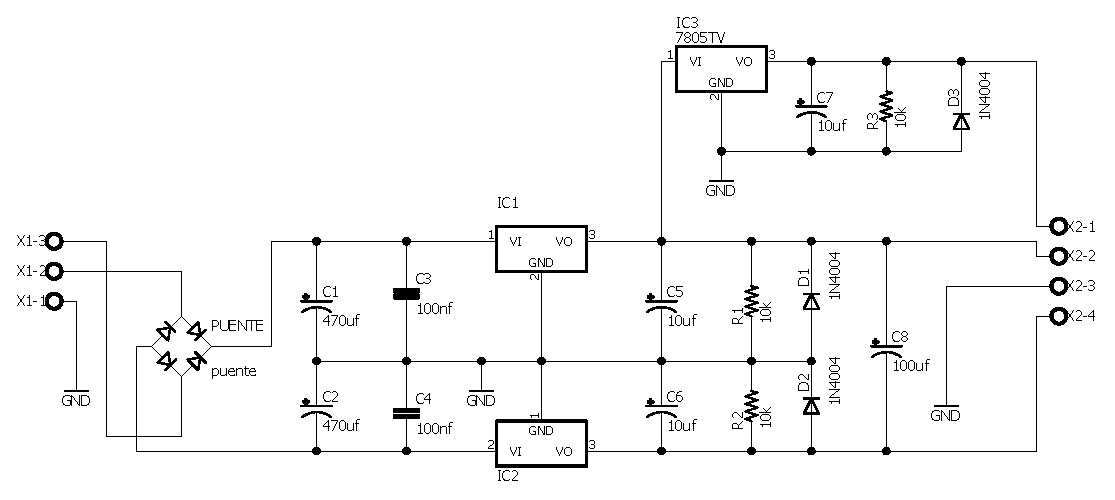
\includegraphics[width=\textwidth]{CircuitoFuente.eps}\caption{Circuito esquemático de la fuente}\label{CircuitoFuente}
\end{figure}
\begin{figure}[]
	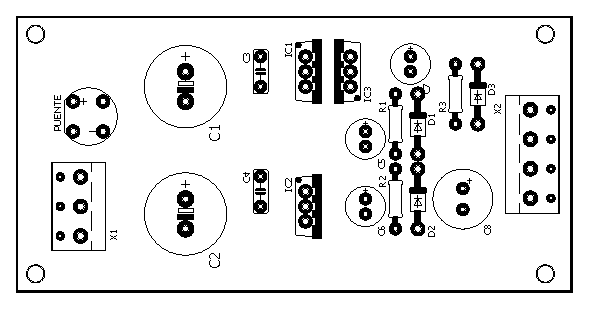
\includegraphics[width=\textwidth]{VistaComponentes.eps};
	 \caption{fuente}\label{LadoComponentesFuente}
\end{figure}

Se puede observar que la fuente consta de tres valores de tensión de salida para que los alumnos tengan al finalizar el trabajo una herramienta versatil. Existe un documento para ampliar la información necesaria para llevar a cabo la construcción de la fuente en el blog de la escuela.

\section{Placa Principal}
La placa principal es el entrenador propiamente dicho y consta a su vez de dos partes; la paca base y la placa superior. Ambas placas son producidas por los alumnos del 7mo año de la carrera en el marco del plan de prácticas internas dentro del laboratorio de diseño electrónico.
\subsection{Circuito Esquemático}
El circuito esta separado en bloques para facilitar su comprensión, ambas placas, tanto la superior como la base se encuentran dentro del mismo circuito esquemático, por esto se podrán observar diferentes tensiones de alimentación que estarán referidas a las distintas placas. También es importante comprender que debido a que ambas placas pueden funcionar separadas, ambas placas tienen conexiones de masa independientes. Algunas partes del circuito son totalmente independientes y requieren se conecte una alimentación externa para operar, es el caso de los potenciómetros, que están pensados para ser utilizados en conjunto con los ADC (conversor analógico a digital). Se puede acceder al circuito completo en la figura \ref{CircuitoEntrenador}. %
\begin{sidewaysfigure}[htb]
	\centering\includegraphics[trim =3cm 0cm 0.5cm 0.5cm, width=0.8\paperheight]{EsquematicoEntrenador};
	\caption{Circuito Esquemático Entrenador Digital}
	\label{CircuitoEntrenador}
\end{sidewaysfigure}%
\subsection{Detalles del impreso y de los componentes}
Se puede observar en la figura \ref{ComponentesEntrenador} los valores y la referencia de cada componente, para completar la información de los componentes más complejos como ser conectores (USB o tiras de pines macho/hembra) consulte la figura \ref{posterEntrenador} o la tabla con la lista de componentes a que se puede consultar en el cuadro \ref{ComponentesEntrenador} . 
\begin{sidewaysfigure}[htb]
	\centering\includegraphics[trim =0cm 0.5cm 0.5cm 0cm, width=0.8\paperheight]{ComponentesEntrenador}	\caption{Vista superior de los componentes del entrenador digital}\label{ComponentesEntrenador}
\end{sidewaysfigure}%
\begin{figure}[htb]
	\centering\includegraphics[width=\textwidth]{PistasEntrenador}	\caption{Vista inferior detalle de las pistas del entrenador digital}\label{PistaEntrenador}
\end{figure}%	
\begin{table}[htb]
	\begin{tabular}{|p{0.3\textwidth}|p{0.1\textwidth}|p{0.18\textwidth}|p{0.3\textwidth}|}
		\hline
		\textbf{Referencia} & \multicolumn{1}{l|}{\textbf{Cantidad}} & \textbf{Valor} & \textbf{Encapsulado} / Tipo \\ \hline
		C10 C9 & 2 & 22pf & Cerámico \\ \hline
		C11 & 1 & 1uf & Electrolitico \\ \hline
		C6 & 1 & 10uf & Electrolitico \\ \hline
		C7 & 1 & 100nf & Cerámico \\ \hline
		C8 & 1 & 47uf & Electrolitico \\ \hline
		D1 D12 & 2 & 1n4004 &  \\ \hline
		D11 D10 D9 D8 D7 D6 D5 
		D4 D3 D2 & 10 & LED & LED\_D3.0mm \\ \hline
		J11 & 1 & LEDS & 1x08\_Pitch2.54mm \\ \hline
		J3 & 1 & ICSP & 1x06\_Pitch2.54mm \\ \hline
		J5 J6 J7 & 3 & CON8 & 1x08\_Pitch2.54mm \\ \hline
		J9 & 1 & 3vias & 1x03\_Pitch2.54mm \\ \hline
		JP1 & 1 & JUMPER3 & 1x03\_Pitch2.54mm \\ \hline
		P1 & 1 & CONN\_01X04 & 1x04\_Pitch2.54mm \\ \hline
		P10 & 1 & Negativo & 1x04\_Pitch2.54mm \\ \hline
		P2 & 1 & DISPLAY & 1x04\_Pitch2.54mm \\ \hline
		P3 & 1 & CONN\_01X05 & 1x05\_Pitch2.54mm \\ \hline
		P4 & 1 & BOTONES & 1x04\_Pitch2.54mm \\ \hline
		P5 & 1 & CONN\_01X09 & 1x09\_Pitch2.54mm \\ \hline
		P6 & 1 & USB\_B & USB\_B \\ \hline
		P7 & 1 & 12V & Bornera 2 bornes \\ \hline
		P8 & 1 & 5V & Bornera 2 bornes \\ \hline
		P9 & 1 & Positivo & 1x04\_Pitch2.54mm \\ \hline
		Q4 Q3 Q2 Q1 & 4 & BC548 & TO-92 \\ \hline
		R20 R19 R18 R17 & 4 & 1200 & R\_Axial\_DIN0207 \\ \hline
		R27 R26 R25 R24 R23 R22 
		R21 R16 R15 R14 R13 R12 
		R11 R10 R9 R28 & 16 & 180 & R\_Axial\_DIN0207 \\ \hline
		R3 R4 & 2 & 470 & R\_Axial\_DIN0207 \\ \hline
		R32 R31 R30 R29 & 4 & 10k & R\_Axial\_DIN0207 \\ \hline
		R8 R7 R6 R5 R1 R2 & 6 & 10K & R\_Axial\_DIN0207 \\ \hline
		RV1 RV2 & 2 & 10K lin & Potenciómetro \\ \hline
		S6 S5 S4 S3 S2 S1 & 6 & SW DPST\_2 & Pulsador \\ \hline
		U1 & 1 & CC56-12EWA & 4display 7 seg cátodo común \\ \hline
		U2 & 1 & ULN2803 & DIP-18 \\ \hline
		U3 & 1 & CD4511 & DIP-16 \\ \hline
		U4 & 1 & LM7805 & TO-220-3\_Vertical \\ \hline
		U5 & 1 & PIC18F4550-I/P & DIP-40 \\ \hline
		Y2 & 1 & 20MHz & Crystal\_HC49-4H \\ \hline
	\end{tabular}
	\caption{Lista de Componentes}
	\label{ListaComponentes}
\end{table}
\pagebreak%
\subsection{Aspecto de la placa}
Finalizada la placa, la misma deberá tener un aspecto como se puede observar en la imagen renderizada de la figura \ref{posterEntrenador} . 
\begin{figure}[htb]

	\centering\includegraphics[width=0.9\textwidth,clip=true]{Entrenador1-SchDoc_4Display_en_uno}

	\caption{Vista de ambas placas (superior y base) del entrenador con sus componentes ya instalados}\label{posterEntrenador}
\end{figure}



	




